\documentclass[tikz,border=10pt]{standalone}
\usepackage{amsmath,amssymb}
\usepackage{pgfplots}
\pgfplotsset{compat=1.18}
\usetikzlibrary{arrows.meta,positioning,calc,decorations.pathmorphing,shapes}

\definecolor{politoNavy}{RGB}{0, 43, 91}
\definecolor{deepdiveTeal}{RGB}{0, 128, 128}
\definecolor{examred}{RGB}{180, 40, 40}
\definecolor{intuitiongreen}{RGB}{40, 130, 80}
\definecolor{fogGray}{RGB}{220, 225, 235}

\begin{document}
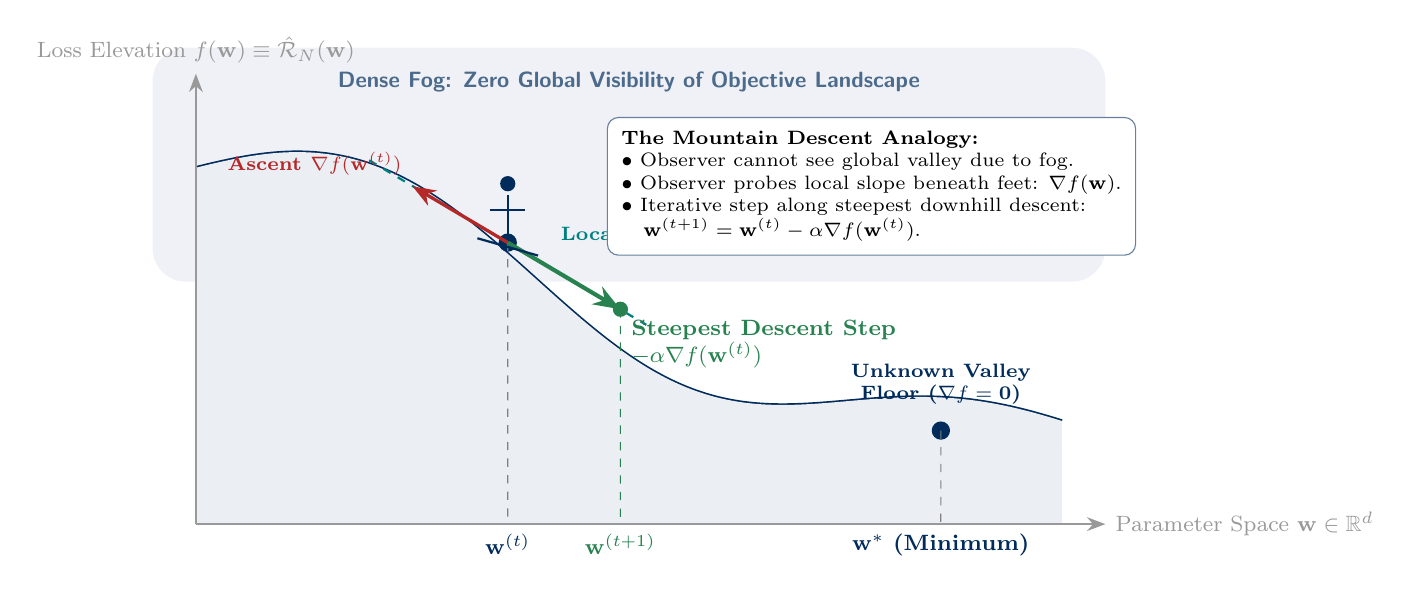
\begin{tikzpicture}[>=Stealth, scale=1.1]
  % Background Fog/Clouds
  \fill[fogGray, opacity=0.45, rounded corners=12pt] (-0.5, 2.8) rectangle (10.5, 5.5);
  \node[font=\sffamily\footnotesize\bfseries, text=politoNavy!70] at (5.0, 5.1) {Dense Fog: Zero Global Visibility of Objective Landscape};

  % Terrain Profile (smooth non-convex mountain slope)
  \draw[very thick, politoNavy, domain=0:10, samples=200, smooth] 
    plot (\x, {1.0 + 3.2/(1 + exp((\x - 4.5)*0.8)) + 0.35*sin(180*\x/3.5)});

  % Shading under terrain
  \fill[politoNavy!8, domain=0:10, samples=200]
    (0,0) -- plot (\x, {1.0 + 3.2/(1 + exp((\x - 4.5)*0.8)) + 0.35*sin(180*\x/3.5)}) -- (10,0) -- cycle;

  % Axes / baseline
  \draw[->, thick, gray!80] (0,0) -- (10.5,0) node[right, font=\footnotesize] {Parameter Space $\mathbf{w} \in \mathbb{R}^d$};
  \draw[->, thick, gray!80] (0,0) -- (0,5.2) node[above, font=\footnotesize] {Loss Elevation $f(\mathbf{w}) \equiv \hat{\mathcal{R}}_N(\mathbf{w})$};

  % Current position w^(t) at x = 3.6
  % y(3.6) approx: 1.0 + 3.2/(1 + exp(-0.9*0.8)) + 0.35*sin(180*3.6/3.5)
  % Let's define the point on curve
  \coordinate (WT) at (3.6, 3.25);
  \fill[politoNavy] (WT) circle (3pt);
  \draw[dashed, thin, gray] (WT) -- (3.6, 0) node[below, font=\footnotesize\bfseries, text=politoNavy] {$\mathbf{w}^{(t)}$};

  % Tangent line at w^(t)
  \draw[thick, dashed, deepdiveTeal] ($(WT) + (-1.6, 0.95)$) -- ($(WT) + (1.6, -0.95)$);
  \node[font=\scriptsize\bfseries, text=deepdiveTeal, above right] at ($(WT) + (0.5, -0.15)$) {Local Slope $\nabla f(\mathbf{w}^{(t)})$};

  % Uphill gradient vector
  \draw[->, very thick, examred] (WT) -- ($(WT) + (-1.1, 0.65)$) 
    node[above left, font=\scriptsize\bfseries, text=examred] {Ascent $\nabla f(\mathbf{w}^{(t)})$};

  % Downhill step vector
  \draw[->, line width=1.5pt, intuitiongreen] (WT) -- ($(WT) + (1.3, -0.77)$)
    node[below right, font=\footnotesize\bfseries, text=intuitiongreen, align=left] {Steepest Descent Step\\$-\alpha \nabla f(\mathbf{w}^{(t)})$};

  % Next point w^(t+1)
  \coordinate (WTP1) at ($(WT) + (1.3, -0.77)$);
  \fill[intuitiongreen] (WTP1) circle (2.5pt);
  \draw[dashed, thin, intuitiongreen] (WTP1) -- (4.9, 0) node[below, font=\footnotesize\bfseries, text=intuitiongreen] {$\mathbf{w}^{(t+1)}$};

  % Valley / Goal Minimum at x = 8.5
  \coordinate (WMIN) at (8.6, 1.08);
  \fill[politoNavy] (WMIN) circle (3pt);
  \draw[dashed, thin, gray] (WMIN) -- (8.6, 0) node[below, font=\footnotesize\bfseries, text=politoNavy] {$\mathbf{w}^*$ (Minimum)};
  \node[above=6pt, font=\scriptsize\bfseries, text=politoNavy, align=center] at (WMIN) {Unknown Valley\\Floor ($\nabla f = \mathbf{0}$)};

  % Stylized Skier / Observer at WT
  \draw[thick, politoNavy] ($(WT) + (0, 0.1)$) -- ($(WT) + (0, 0.55)$); % body
  \fill[politoNavy] ($(WT) + (0, 0.68)$) circle (2.5pt); % head
  \draw[thick, politoNavy] ($(WT) + (-0.2, 0.38)$) -- ($(WT) + (0.2, 0.38)$); % arms
  \draw[thick, politoNavy] ($(WT) + (-0.35, 0.05)$) -- ($(WT) + (0.35, -0.15)$); % ski on slope

  % Pedagogical Callout Box
  \node[draw=politoNavy!60, fill=white, rounded corners=4pt, font=\scriptsize, align=left, inner sep=5pt] at (7.8, 3.9) {
    \textbf{The Mountain Descent Analogy:}\\
    $\bullet$ Observer cannot see global valley due to fog.\\
    $\bullet$ Observer probes local slope beneath feet: $\nabla f(\mathbf{w})$.\\
    $\bullet$ Iterative step along steepest downhill descent:\\
    \quad $\mathbf{w}^{(t+1)} = \mathbf{w}^{(t)} - \alpha \nabla f(\mathbf{w}^{(t)})$.
  };
\end{tikzpicture}
\end{document}
